\clearpage
\chapter{Engenharia de Software}

Este capítulo contém o referencial teórico que diz respeito à Engenharia de Software utilizada nesse trabalho.

\section{\textit{Framework} de gerenciamento \textit{SCRUM}}

O \textit{SCRUM} é um \textit{framework} de gerenciamento de projetos cuja característica principal é o desenvolvimento de um produto complexo e tem como objetivo entregar o produto com o maior valor agregado possível \cite{sutherland1995}.

Segundo \citeonline{sutherland1995} os três pilares que sustentam o \textit{SCRUM} são:

\begin{itemize}
    \item \textbf{Transparência:} manter os resultados sempre visíveis aos interessados, para que todos possam ter um mesmo ponto de vista.
    \item \textbf{Inspeção:} deve-se, frequentemente, inspecionar os artefatos gerados, desde que esse processo não atrapalhe o real trabalho.
    \item \textbf{Adaptação:} uma vez encontrado um erro em qualquer artefato, deve-se ajustar o mesmo o mais rápido possível, para evitar maiores erros.
\end{itemize}

\subsection{Time \textit{SCRUM}}

O time \textit{SCRUM} é formado por três partes distintas: o \textit{product owner}, o time de desenvolvimento e o \textit{scrum master} \cite{sutherland2013}.

\subsubsection{\textit{Product Owner}}
Responsável por manter os itens no \textit{backlog} do produto, tornando ele visível e claro a todos, garantindo que o time de desenvolvimento entenda-os.

\subsubsection{Time de Desenvolvimento}
Composto por desenvolvedores, o time de desenvolvimento é responsável por transformar o \textit{backlog} do produto em incrementos de software.

\subsubsection{\textit{Scrum Master}}
É o responsável pelo cumprimento das práticas do \textit{SCRUM}, facilitando os eventos propostos pelo \textit{framework}, trabalhando em conjunto com o \textit{product owner} para o esclarecimentos dos itens do \textit{backlog} para a equipe de desenvolvimento, além de liderar o time em seu autogerenciamento.

\subsection{Eventos do \textit{SCRUM}}

No \textit{SCRUM}, todos os eventos possuem uma duração determinada, que varia de acordo com a necessidade do projeto e equipe. São eles: \textit{sprint}, reunião de planejamento de \textit{sprint} e revisão da \textit{sprint} \cite{sutherland2013}.

\subsubsection{\textit{Sprint}}
A \textit{sprint} é o evento mais importante, pois ela agrupa todos os outros eventos. Uma \textit{sprint} possui um tempo fixo, que pode variar de acordo com a necessidade da equipe, e pode ser composta de outras atividades e eventos do \textit{SCRUM}, como reuniões diárias, desenvolvimento do produto, retrospectivas, etc. Uma \textit{sprint} sempre começa quando uma acaba \cite{sutherland2013}.

\subsubsection{Reunião de planejamento de \textit{sprint}}
Ocorre sempre no início de cada \textit{sprint} e, como resultado da reunião, é definido o que será feito durante a \textit{sprint} que se inicia. A partir disso, é criado o \textit{backlog} de \textit{sprint}, onde estão presentes as metas da \textit{sprint}.

\subsubsection{Revisão de \textit{sprint}}
Acontece no final de cada \textit{sprint} e tem como objetivo a apresentação dos resultados obtidos durante a \textit{sprint} que passou, tanto o que foi concluído quanto o que não foi, bem como as justificativas para a não completude. Nessa reunião, todos os membros do time devem estar presentes.

\subsection{Artefatos do \textit{SCRUM}}
Durante o andamento do projeto, alguns artefatos são produzidos, com o objetivo de guiar a equipe e facilitar o entendimento comum entre todos os envolvidos \cite{sutherland2013}.

\subsubsection{\textit{Backlog} de produto}
É uma lista com todas as atividades que precisam ser feitas para que o produto final seja concluído. Essa lista evoluí junto com o projeto, uma característica do modelo de desenvolvimento iterativo e incremental.

\subsubsection{\textit{Backlog} de \textit{sprint}}
Assim como o \textit{backlog} de produto, porém com um escopo menor. O \textit{backlog} de \textit{sprint} lista todas as atividades que foram planejadas para uma determinada \textit{sprint}.

\section{Testes de Software}
O desenvolvimento de software é uma atividade que envolve várias atividades e, muitas vezes, diferentes pessoas, o que acaba por favorecer a inserção de defeitos no produto. Além disso, o mal entendimento dos requisitos pode resultar na produção de algo que não foi solicitado pelo cliente \cite{trodo2009}.

Os testes de software representam, então, uma atividade que compõe o processo de verificação de validação do software e consiste em uma análise dinâmica do código-fonte, ou seja, o código deve ser executado para que os testes possam ocorrer. Isso possibilita a identificação de erros, bem como a prevenção de inserção de novos erros, quando os testes são automatizados \cite{barbosa2009}.

\subsection{Classificação dos Testes}
Os testes de software podem ser classificados, dentre outras categorias, em testes de caixa-preta e testes de caixa-branca \cite{barbosa2009}.

\subsubsection{Testes de caixa-preta}
Esse tipo de teste tem como objetivo avaliar o produto em relação aos requisitos funcionais e não-funcionais. A figura abaixo mostra o funcionamento de um teste de caixa-preta, onde são utilizados determinados dados de entrada no software e os resultados obtidos são comparados com as expectativas para os dados de entrada \cite{barbosa2009}.

\begin{figure}[h]
  \centering
  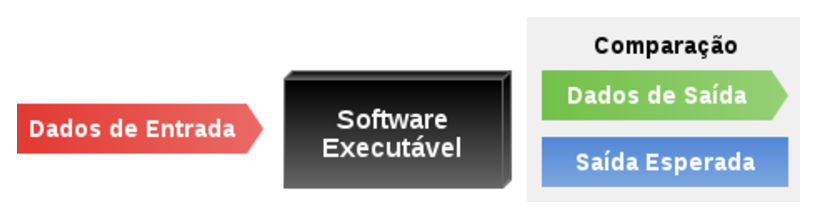
\includegraphics[scale=0.7]{figuras/caixa-preta.eps}
  \caption{Representação do teste de caixa-preta}
\end{figure}